\chapter{Data and analysis}

For this project we make use of good quality deep data of galaxy clusters observed with the MegaCam wide field imager on the CFHT (Canada-France-Hawii Telescope). The cluster sample consisted of 101 clusters within the range of redshifts from $0.05<z<0.55$. The full description of this survey can be found in: D. J. Sand et. al. \citeyear{Reference11}

58 clusters from the MENEACS (Multi-Epoch Nearby Cluster Survey). The MENEACS clusters represent all clusters in the BAX X-ray cluster database that are observable for the CFHT and this part of the data is in the G and R bands. We also make use of the INT data of the same cluster in the bands I and U. 

After filtering out some of the clusters because of a very complex and crowded central region or just not good quality we used 30 clusters for the final studies and paid special attention to 10, marked with * in table 4.1.

The original images have dimensions of [11000:11000] pixels but since our relevant region is the center of the cluster where the BCG is located, we cut the images with dimension of [1000,1000] for the color analysis and [4000:4000] to characterize the colors and discriminate between cluster and non-cluster members.

\begin{table}[H]
\centering

\begin{tabular}{ccccc}
Cluster & $z$   & $\sigma(km/s)$ & $d(Mpc)$ & $\theta_{E}(")$ \\ \hline \hline
A1033   & 0.126 & 762            & 540 & 14.6155  \\
A1068*  & 0.138 & 740            & 591.4 & 13.5945  \\
A1132   & 0.136 & 727            & 582.9 & 13.1515   \\
A119*   & 0.044 & 875            & 188.6 & 21.0798   \\
A1413*  & 0.143 & 881            & 612.9 & 19.1569   \\
A1650   & 0.084 & 720            & 360 & 13.6758   \\
A1651   & 0.085 & 903            & 364.3 & 21.4876   \\
A1795   & 0.062 & 778            & 265.7 & 16.3514   \\
A2029*  & 0.077 & 1152           & 330 & 35.2776   \\
A2050   & 0.118 & 854            & 505.7 & 18.5258   \\
A2055   & 0.102 & 697            & 437.1 & 12.5642   \\
A2064   & 0.108 & 675            & 462.9 & 11.7048   \\
A2065*  & 0.073 & 1095           & 312.9 & 32.0110   \\
A2069   & 0.116 & 966            & 497.1 & 23.7574   \\
A2142*  & 0.091 & 1086           & 390 & 30.8756   \\
A2319*  & 0.056 & 1101           & 240 & 32.9563   \\
A2420   & 0.085 & ~800           & 364.3 & 16.8653   \\
A2440   & 0.091 & 766            & 390 & 15.3608   \\
A2597   & 0.085 & 682            & 364.3 & 12.2569   \\
A2627   & 0.126 & ~800           & 540 & 16.1096   \\
A2703   & 0.114 & ~800           & 488.6 & 16.3307   \\
A399    & 0.072 & ~800           & 308.6 & 17.1049   \\
A553    & 0.066 & ~800           & 282.9 & 17.2155   \\
A655*   & 0.127 & ~800           & 544.3 & 16.0911   \\
A754*   & 0.054 & ~800           & 231.4 & 17.4367   \\
A763    & 0.085 & ~800           & 364.3 & 16.8653   \\
A795    & 0.136 & ~800           & 582.9 & 15.9252   \\
A85*    & 0.055 & ~800           & 235.7 & 17.4182   \\
A961    & 0.124 & ~800           & 531.4 & 16.1464   \\
A990    & 0.144 & ~800           & 617.1 & 15.7778   
\end{tabular}
\caption[Abell Clusters and their redshift]{Abell clusters used in this work. Marked with * the chosen clusters with the most promising features. From left to right: Name of the cluster, redshift, velocity dispersions from C. Bildfell et. al. \citeyear{Reference6}, distance in Mpc and Einstein Ring using a single isothermal sphere as first approximation.}
\end{table}

The INT images were obtained using multiple exposures so it was necessary to make a mosaic of them using \texttt{SWARP}, so at the end we had the data of the clusters in the bands G,R,U,I with the same spatial scale. The first step in the removal of the light from the BCG was constructing a mask file (segmentation file) to only extract the desired galaxy, this was done using \texttt{SEXTRACTOR} (Bertin, E. \& Arnouts, S \citeyear{Reference27}). 

The procedure is the following: \texttt{SEXTRACTOR} identifies the bright objects and extracts them while doing aperture photometry on them, the user can choose to obtain an examination image to see the extracted objects (that in our case would be the segmentation file). \texttt{SEXTRACTOR} labels each of the extracted regions with growing numbers where 1 is the brightest object (in most cases the BCG) so we can use python scripts to modify the segmentation file to mask only the galaxies but not the BCG which we want to fit properly. Figure [4.1] shows the original segmentation image and the one where the BCG light has been removed so that it won't be masked once we fit the light of the BCG. 

\begin{figure}[H]
\centering
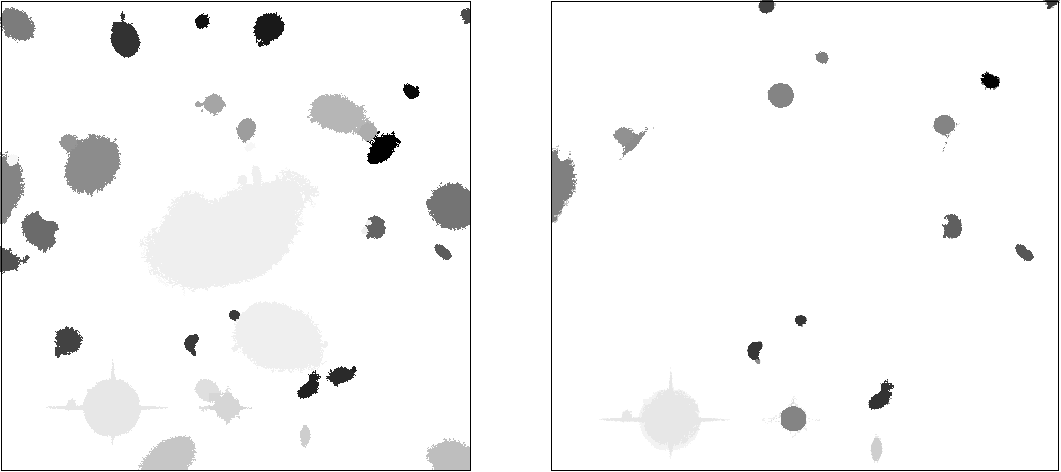
\includegraphics[width=15cm]{images/masks.png}
\caption[Segmentation images]{Segmentation images produced by \texttt{SEXTRACTOR} and used as mask files for the galfit extraction. Left panel is the original mask with all the bright objects. Right panel is the mask after the subtraction of the regions surrounding the cluster galaxies to be fitted with \texttt{GALFIT}. The colors are inverted for an easier visualization of the image. The fainter regions are actually the most luminous objects because \texttt{GALFIT} assigns increasing numbers starting from the brightest one, that is the BCG in this case}
\end{figure}

Now, once the mask file is ready we can do the substraction of the BCG light using \texttt{GALFIT} (Peng et. al \citeyear{Reference20}) which fits two dimensional profiles of galaxies (with different shapes and features). The first subtraction for most of our target clusters was done fitting a Sersic's profile with n=4 which is de Vaucouleurs profile. Although in all cases some parameters such as the $n$ index, the effective radius, Fourier and bending modes were to be changed and modified accordingly. A first run of \texttt{GALFIT} gives us a rough idea of the true position of the center of the BCG so we can set this values in a second run for each cluster. 

We use the segmentation masks given by \texttt{SEXTRACTOR} to mask bright objects in the fitting of the BCG but in some cases it was necessary to do the fitting of many objects (not only the BCG). The best results were given when we also masked the innermost region of the BCG (the size of the seeing) so the fitting will put more weight in the rest of the profile, thus reducing most of the light that hides the background objects.

The power of \texttt{GALFIT} lies in the fact that it allows for different shape fitting through fourier and bending modes. These parameters (\texttt{C0, B1, B2, F1, F2}, etc.) are hidden from the user unless he/she explicitly requests them.  These can be tagged on to the end of any previous components except, of course, the PSF and the sky.  

Some of the useful parameters that we used to properly fit the BCG in every case were: \texttt{B1)} Bending mode 1 (shear term), \texttt{B2)} Bending mode 2 (banana shape)
\texttt{B3)} Bending mode 3 (S-shape) and for the azimuthal fourier modes
\texttt{F$_i$)} Az. Fourier mode $i$ where $i$ can go up to a 20th Fourier mode, \texttt{C0)}   traditional diskyness(-)/boxyness(+).

Figure [4.2] shows the original image, the fitted models and the output given by \texttt{GALFIT} for the cluster ABELL754. Note that many galaxies were fitted and many background objects can be seen near the center of the BCG. 

\begin{figure}[H]
\centering
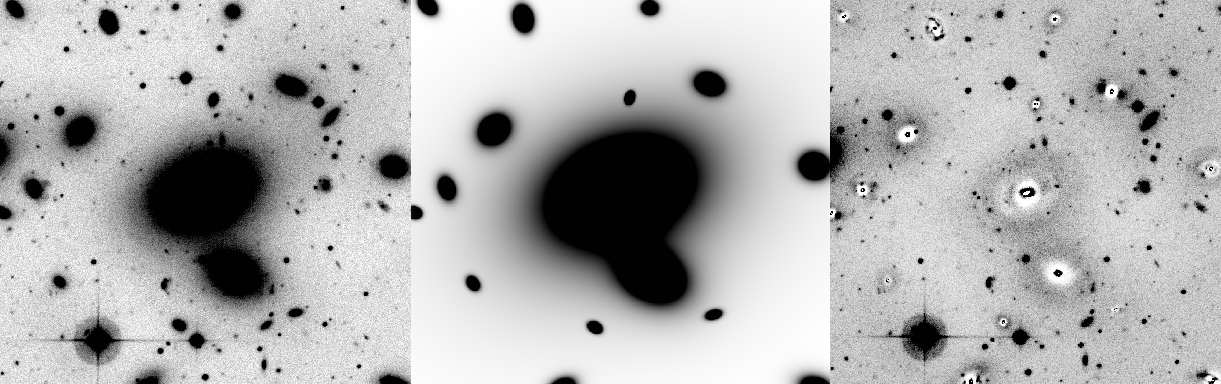
\includegraphics[width=15cm]{images/galfit.png}
\caption[Galfit results]{Galfit procedures. Left: Original image in ``zscale" with the clear BCG expanding across a significant region of the central area. Middle: The models fitted by \texttt{GALFIT} for all the selected cluster galaxies. Right: Residual image after the subtraction of the model galaxies.}
\end{figure}


The same for cluster ABELL1413:

\begin{figure}[H]
\centering
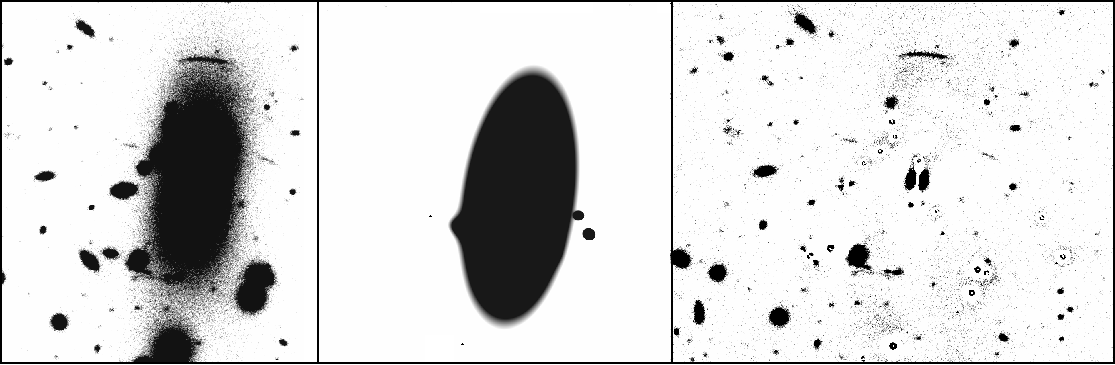
\includegraphics[width=15cm]{images/A1413.png}
\caption[Galfit results]{Galfit procedures on A1413. Left: Original image in ``zscale" with the clear BCG expanding across a significant region of the central area. Middle: The models fitted by \texttt{GALFIT} for all the selected cluster galaxies. Right: Residual image after the subtraction of the model galaxies.}
\end{figure}

\section{Color images} 

We use \texttt{IRAF} to make the color images using our G,R,U,I bands. Let's keep using ABELL754 which is a low redshift galaxy ($z=0.054$) cluster with a calculated mass of $\text{M}_{200}=9.8\times 10^{15} \text{M}_{\odot}$ (Sifon et. al. \citeyear{Reference9})

Here we take an isothermal sphere to model the Einstein ring for an assumed distance of background objects of $z=0.5$. We made a color image of the original center of the cluster without subtracting the BCG in order to differentiate between cluster members from background galaxies and field stars. This allows us to fit only the cluster galaxies. 

\begin{figure}[H]
\centering
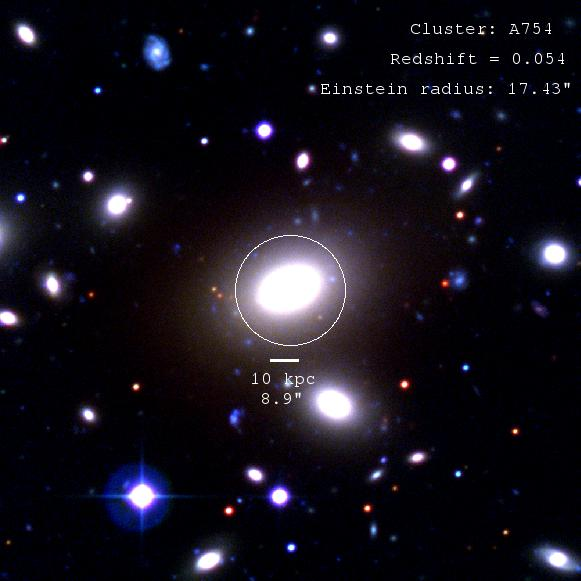
\includegraphics[width=12cm]{images/cA754.jpg}
\caption[Color image of A754]{Color image of A754 cluster (filters I,G,U) with its Einstein radius calculated for an isothermal sphere of a background object at $z=1$.}
\end{figure}

After choosing the galaxies that belong to the cluster by comparing their relative colors, we subtracted them using \texttt{GALFIT} and made the color image again changing the scaling values with the task \texttt{CONVERT} of \texttt{IRAF} so that we see can see the color contrast to search for good candidates of lensed objects. By looking at this reduced color image, we have another visual constraint to choose the clusters in which it would be worth to do photometric redshifts and search for objects with the same redshift in different locations around the very center of the BCG (object that has suffered strong lensing). 

\begin{figure}[H]
\centering
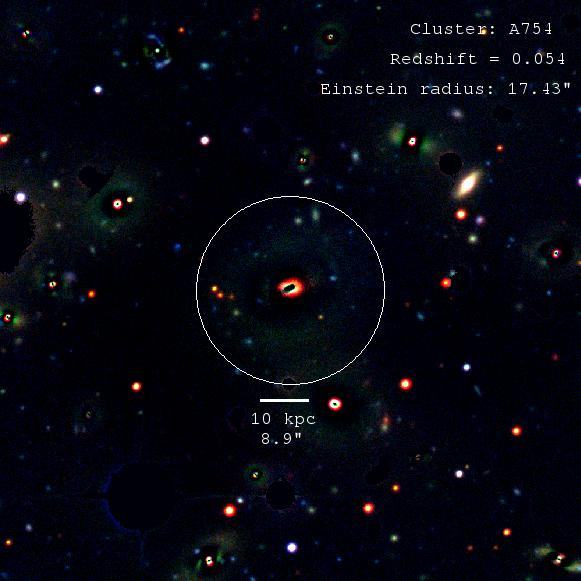
\includegraphics[width=12cm]{images/cA754_galfit.jpg}
\caption[Color image of A754 after fitting the bright objects]{Color image of A754 cluster (filters I,G,U) after the subtraction of the bright cluster galaxies.}
\end{figure}

Because we have 4 bands we were able to make different color images to see the contrast and make combinations that would allow us to see better the very red and very blue objects, hoping to find objects with the same colors that would be good candidates for lensed objects. Figure [4.5] displays the G-R, I-R-G and I-G-U color images for three clusters (ABELL961, ABELL2703 and ABELL1033). 

\begin{figure}[H]
\centering
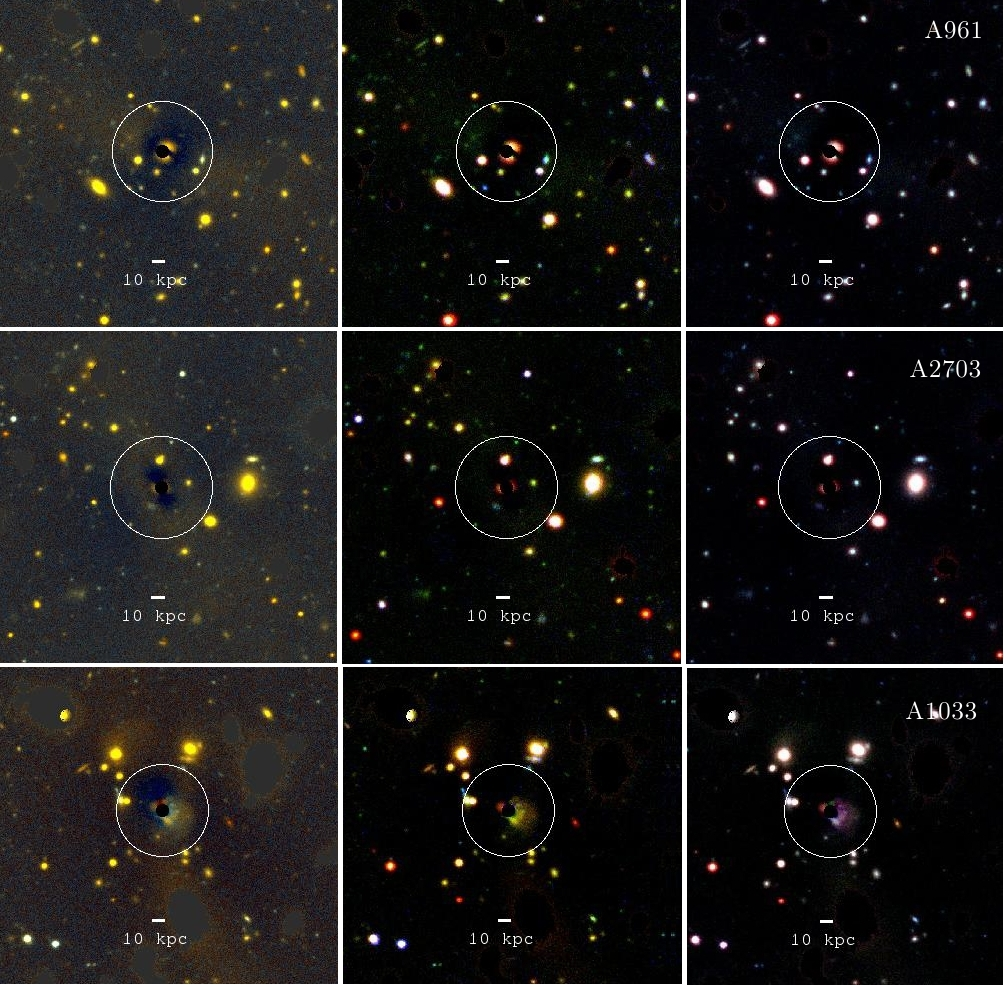
\includegraphics[width=15cm]{images/full_small.jpg}
\caption[Color images for various clusters]{Different color images for different combination of the G,R,U,I filters for the clusters A961, A2703, A1033. Left column for the images constructed only with the g and r filter, central column for i,g,r and right column for I,G,U.}
\end{figure}

\section{Photometric Redshifts}

The first step in determining the photometric redshifts is to discriminate between field stars and the galaxies of the clusters so in order to do this, we used some of the parameters found by \texttt{SEXTRACTOR} that allow us to constraint the fitted data. These are \texttt{class-star}, \texttt{flux\_radius}, and \texttt{FWHM} (full wicth half maximum). Class-star uses the neural network star/galaxy of \texttt{SEXTRACTOR} that will give values close to 1 for stars and 0 for galaxies. \texttt{flux\_radius}, and \texttt{FWHM} are closely related to each other and give the radius which contains half of the light of the object so it will be small for stars and bigger for extended objects.

In order to extract the same objects and make the segmentation masks for the desired objects in the different filters, we used \texttt{SEXTRACTOR} on dual mode and made aperture photometry on each of the relevant objects. Figure [4.6] shows the color magnitude diagram for ABELL754 where we used a zero point magnitude of 30.

\begin{figure}[H]
\centering
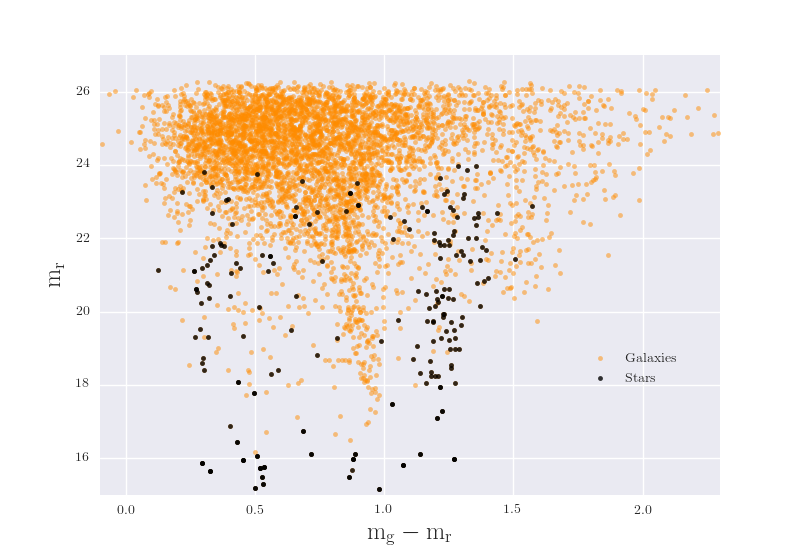
\includegraphics[width=12cm]{images/color_mag.png}
\caption[Color Magnitude diagram of ABELL754]{Color Magnitude diagram of ABELL1068 with the differentiation of stars from galaxies}
\end{figure}

We can also discriminate the stars from galaxies using the radius that contains most of the flux. Figure [4.7] shows the galaxies and stars in the Mag vs \texttt{Flux\_rad} plane.

\begin{figure}[H]
\centering
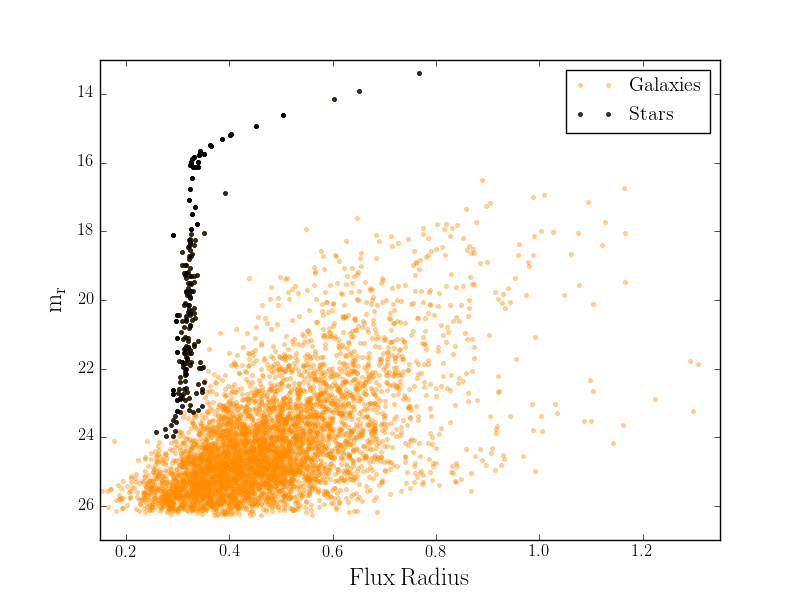
\includegraphics[width=12cm]{images/mag_vs_flux_rad.png}
\caption[Magnitude vs Flux radius of ABELL754]{Magnitude vs Flux radius of ABELL1068 to identify the galaxies using the criteria of their flux distribution}
\end{figure}

Once we have selected only the magnitudes of the galaxies in our four filters, we can measure the photometric redshift of the galaxies in the inner region of the cluster after the subtraction of the BCG, we use the photometric redshift code \texttt{EAZY} (Brammer et. al 2008) which uses an extensive collection of spectral energy distributions for galaxies in the range $0<z<4$. Fortunately, the code includes library from CFHT in the I and U bands but doesn't have the filters in the G and R bands so I used the SUBARU survey filter information to be able to compute the photometric redshifts using four bands.

citation of \texttt{EAZY} ``Brammer, van Dokkum and Coppi, \citeyear{Reference22}" 
